% ============================================================
% Diagram Lingkaran untuk Statistika SMP - pendamping artikel blog
% https://pakgun.gezytech.web.id/tikz-diagram-lingkaran-statistika/
% Kompilasi: pdflatex (standalone, butuh paket tikz)
% Ganti frekuensinya, sudut dihitung otomatis oleh pgfmath.
% ============================================================
\documentclass[tikz,border=10pt]{standalone}
\begin{document}
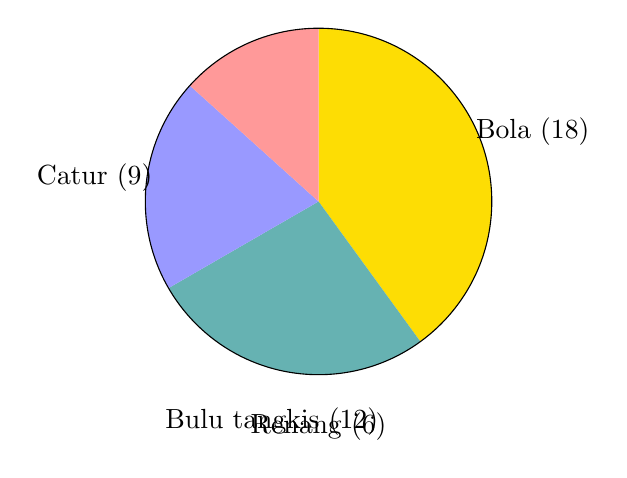
\begin{tikzpicture}[scale=1.1]
  % hitung sudut dengan pgfmath supaya presisi
  \newcommand{\total}{45}
  \pgfmathsetmacro{\a}{360*18/\total}  % bola: 144
  \pgfmathsetmacro{\b}{360*12/\total}  % bulu tangkis: 96
  \pgfmathsetmacro{\c}{360*9/\total}   % catur: 72
  % sisanya renang: 48

  \fill[yellow!80!orange] (0,0) -- (90:{2}) arc (90:90-\a:{2}) -- cycle;
  \fill[teal!60]          (0,0) -- (90-\a:{2}) arc (90-\a:90-\a-\b:{2}) -- cycle;
  \fill[blue!40]          (0,0) -- (90-\a-\b:{2}) arc (90-\a-\b:90-\a-\b-\c:{2}) -- cycle;
  \fill[red!40]           (0,0) -- (90-\a-\b-\c:{2}) arc (90-\a-\b-\c:-270:{2}) -- cycle;

  \draw (0,0) circle (2);
  \node at (90-\a/2:2.6) {Bola (18)};
  \node at (90-\a-\b/2:2.6) {Bulu tangkis (12)};
  \node at (90-\a-\b-\c/2:2.6) {Catur (9)};
  \node at (270:2.6) {Renang (6)};
\end{tikzpicture}
\end{document}
